\subsection{Нейросетевой анализ}
\label{sec:analysis:neural_networks}

Нейронная сеть (также искусственная нейронная сеть, ИНС) — математическая модель, а также её программное или аппаратное
воплощение, построенная по принципу организации и функционирования биологических нейронных сетей — сетей нервных клеток
живого организма. Это понятие возникло при изучении процессов, протекающих в мозге, и при попытке смоделировать эти
процессы.

Нейронные сети используются для решения сложных задач, которые требуют аналитических вычислений подобных тем, что
делает человеческий мозг. Самыми распространенными применениями нейронных сетей является:

\begin{itemize}
  \item Классификация — распределение данных по параметрам. Например, на вход дается набор людей и нужно решить, кому из них давать кредит, а кому нет. Эту работу может сделать нейронная сеть, анализируя такую информацию как: возраст, платежеспособность, кредитная история и тд.
  \item Предсказание — возможность предсказывать следующий шаг. Например, рост или падение акций, основываясь на ситуации на фондовом рынке.
  \item Распознавание — в настоящее время, самое широкое применение нейронных сетей. Используется в Google, когда вы ищете фото или в камерах телефонов, когда оно определяет положение вашего лица и выделяет его и многое другое.
\end{itemize}

Классификация искусственных нейронных сетей представлена на рисунке~\ref{fig:analysis:neural-classification}

\begin{figure}[!ht]
  \centering
  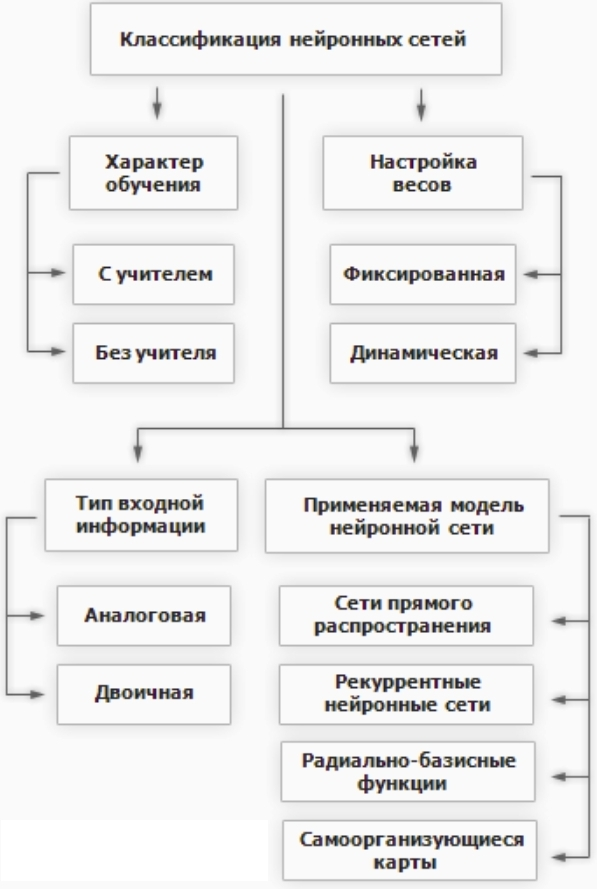
\includegraphics[scale=0.6]{neural-classification.jpg} 
  \caption{Классификация нейронных сетей}
  \label{fig:analysis:neural-classification}
\end{figure}

Задачи прогнозирования (предсказания) можно разбить на два основных класса: классификация и регрессия.

В задачах классификации нужно бывает определить, к какому из \linebreak
нескольких заданных классов принадлежит данный входной
набор. Примерами могут служить предоставление кредита (относится ли данное лицо к группе высокого или низкого
кредитного риска), диагностика раковых заболеваний (опухоль, чисто), распознавание подписи (поддельная, подлинная).
Во всех этих случаях, очевидно, на выходе требуется всего одна номинальная переменная.
Чаще всего (как в этих примерах) задачи классификации бывают двузначными, хотя встречаются и задачи с несколькими
возможными состояниями.

В задачах регрессии требуется предсказать значение переменной, принимающей (как правило) непрерывные числовые
значения: завтрашнюю цену акций, расход топлива в автомобиле, прибыли в следующем году и т.п.. В таких случаях в
качестве выходной требуется одна числовая переменная.

Исскусственные нейронные сети обычно состоят из нейронов и связывающих их синапсов.

\begin{figure}[!ht]
  \centering
  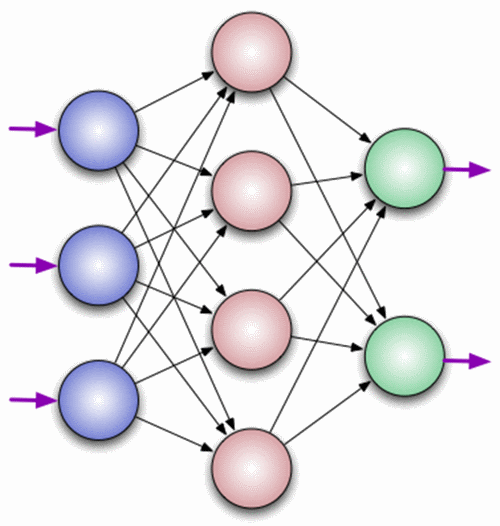
\includegraphics[scale=1]{neurons.png} 
  \caption{Виды нейронов}
  \label{fig:analysis:neurons}
\end{figure}

Нейрон — это вычислительная единица, которая получает информацию, производит над ней простые вычисления и передает ее
дальше. Они делятся на три основных типа: входной (слева), скрытый (посередине) и выходной (справа). Также есть нейрон
смещения и контекстный нейрон. В том случае, когда нейросеть состоит из большого количества нейронов, вводят термин
слоя. Соответственно, есть входной слой, который получает информацию, \emph{n} скрытых слоев (обычно их не больше 3),
которые ее обрабатывают и выходной слой, который выводит результат. У каждого из нейронов есть 2 основных параметра:
входные данные (input data) и выходные данные (output data). В случае входного нейрона: input=output. В остальных,
в поле input попадает суммарная информация всех нейронов с предыдущего слоя, после чего, она нормализуется, с помощью
функции активации и попадает в поле output~\cite{neural-networks}.

Нейрон смещения или bias нейрон — это третий вид нейронов, используемый в большинстве нейросетей. Особенность этого
типа нейронов заключается в том, что его вход и выход всегда равняются 1 и они никогда не имеют входных синапсов.
Нейроны смещения могут, либо присутствовать в нейронной сети по одному на слое, либо полностью отсутствовать,
50/50 быть не может (красным на схеме обозначены веса и нейроны которые размещать нельзя). Соединения у нейронов
смещения такие же, как у обычных нейронов — со всеми нейронами следующего уровня, за исключением того, что синапсов
между двумя bias нейронами быть не может. Следовательно, их можно размещать на входном слое и всех скрытых слоях,
но никак не на выходном слое, так как им попросту не с чем будет формировать связь.

Нейрон смещения нужен для того, чтобы иметь возможность получать выходной результат, путем сдвига графика функции
активации вправо или влево.

Также нейроны смещения помогают в том случае, когда все входные нейроны получают на вход 0 и независимо от того какие
у них веса, они все передадут на следующий слой 0, но не в случае присутствия нейрона смещения.

\begin{figure}[!ht]
  \centering
  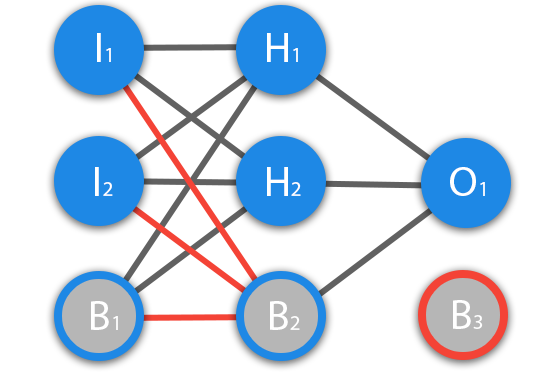
\includegraphics[scale=3]{bias-neurons.png}
  \caption{Нейрон смещения}
  \label{fig:analysis:bias-neurons}
\end{figure}

Синапс -- это связь между двумя нейронами. У синапсов есть 1 параметр — вес. Благодаря ему, входная информация изменяется,
когда передается от одного нейрона к другому. Допустим, есть 3 нейрона, которые передают информацию следующему.
Тогда у нас есть 3 веса, соответствующие каждому из этих нейронов. У того нейрона, у которого вес будет больше, та
информация и будет доминирующей в следующем нейроне (пример — смешение цветов). На самом деле, совокупность весов
нейронной сети или матрица весов — это своеобразный мозг всей системы. Именно благодаря этим весам, входная информация
обрабатывается и превращается в результат.

\begin{figure}[!ht]
  \centering
  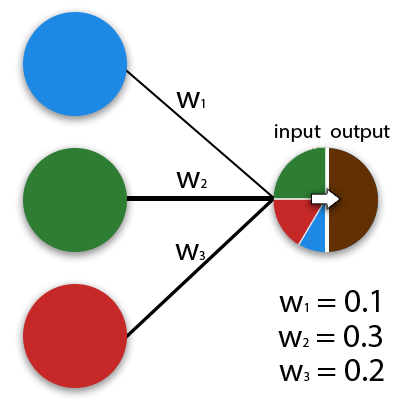
\includegraphics[scale=3]{synaps.png}
  \caption{Синапсы для связи нейронов}
  \label{fig:analysis:synaps}
\end{figure}

Функция активации -- это способ нормализации входных данных. То есть, если на входе у
вас будет большое число, пропустив его через функцию активации, вы получите выход в нужном вам диапазоне. Самые
основные функции активации: Линейная, Сигмоид (Логистическая) и Гиперболический
тангенс. Главные их отличия — это диапазон значений.

Линейная функция почти никогда не используется, за исключением случаев, когда нужно протестировать нейронную сеть или
передать значение без преобразований.

\begin{figure}[!ht]
  \centering
  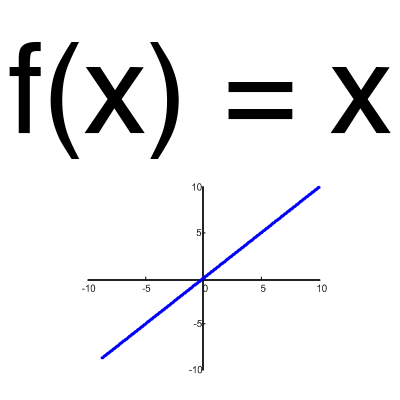
\includegraphics[scale=2.1]{linear-activation.png} 
  \caption{Линейная функция активации}
  \label{fig:analysis:linear-activation}
\end{figure}

Сигмоид -- это самая распространенная функция активации, ее диапазон значений [0,1]. Именно на ней показано большинство примеров
в сети, также ее иногда называют логистической функцией. Соответственно, если в вашем случае присутствуют отрицательные
значения (например, акции могут идти не только вверх, но и вниз), то вам понадобиться функция которая захватывает и
отрицательные значения.

\begin{figure}[!ht]
  \centering
  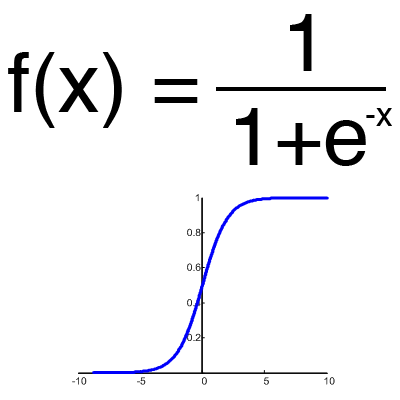
\includegraphics[scale=2.1]{sigmod-activation.png} 
  \caption{Сигмоид}
  \label{fig:analysis:sigmod-activation}
\end{figure}

Имеет смысл использовать гиперболический тангенс, только тогда, когда ваши значения могут быть и отрицательными, и
положительными, так как диапазон функции [-1,1]. Использовать эту функцию только с положительными значениями
нецелесообразно так как это значительно ухудшит результаты вашей нейросети.

\begin{figure}[!ht]
  \centering
  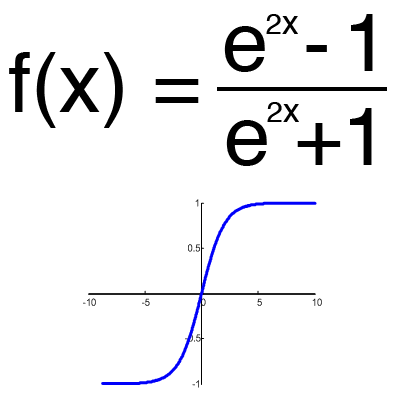
\includegraphics[scale=2.1]{tangens-activation.png} 
  \caption{Гиперболический тангенс}
  \label{fig:analysis:tangens-activation}
\end{figure}

Ошибка — это процентная величина, отражающая расхождение между ожидаемым и полученным ответами. Ошибка формируется
каждую эпоху и должна идти на спад. Ошибку можно вычислить разными путями, например:
Mean Squared Error (далее MSE), Root MSE и Arctan.
Здесь нет какого-либо ограничения на использование, как в функции активации, и можно использовать любой метод, который
будет приносить вам наилучший результат. Стоит лишь учитывать, что каждый метод считает ошибки по разному.
У Arctan, ошибка, почти всегда, будет больше, так как он работает по принципу: чем больше разница, тем больше ошибка.
У Root MSE будет наименьшая ошибка, поэтому, чаще всего, используют MSE, которая сохраняет баланс в вычислении ошибки.

Обучение искусственных нейронных сетей происходит с помощью заранее подготовленной выборки данных (тренировочный сет).

Общее количество тренировочных сетов, пройденных нейронной сетью, называется итерацией.

Эпохой называется количество пройденных наборов тренировочных \linebreak сетов. Чем больше эпоха, тем лучше натренирована сеть и
соответственно, ее результат.

Для получения корректных результатов работы искусственной нейронной сети, её необходимо обучить. Существует несколько
методов обучения нейронных сетей, самые распространенные из них: метод обратного распространения,
метод упругого распространения, генетический алгоритм.

Метод обратного распространения, использует алгоритм градиентного спуска.

Применение алгоритма обратного распространения ошибки — один из известных методов, используемых для глубокого обучения
нейронных сетей прямого распространения (такие сети ещё называют многослойными персептронами). Этот метод относят к
методу обучения с учителем, поэтому требуется задавать в обучающих примерах целевые значения.

Сегодня нейронные сети прямого распространения используются для решения множества сложных задач. Если говорить об
обучении нейронных сетей методом обратного распространения, то тут пользуются двумя проходами по всем слоям нейросети:
прямым и обратным. При выполнении прямого прохода осуществляется подача входного вектора на входной слой сети, после
чего происходит распространение по нейронной сети от слоя к слою. В итоге должна осуществляться генерация набора
выходных сигналов — именно он, по сути, является реакцией нейронной сети на этот входной образ. При прямом проходе все
синаптические веса нейросети фиксированы. При обратном проходе все синаптические веса настраиваются согласно правил
коррекции ошибок, когда фактический выход нейронной сети вычитается из желаемого, что приводит к формированию сигнала
ошибки. Такой сигнал в дальнейшем распространяется по сети, причём направление распространения обратно направлению
синаптических связей. Именно поэтому соответствующий метод и называют алгоритмом с обратно распространённой ошибкой.
Синаптические веса настраивают с целью наибольшего приближения выходного сигнала нейронной сети к желаемому.

Цель обучения нейросети при использовании алгоритма обратного распространения ошибки — это такая подстройка весов
нейросети, которая позволит при приложении некоторого множества входов получить требуемое множество выходов нейронов
(выходных нейронов). Можно назвать эти множества входов и выходов векторами. В процессе обучения предполагается,
что для любого входного вектора существует целевой вектор, парный входному и задающий требуемый выход. Эту пару
называют обучающей. Работая с нейросетями, мы обучаем их на многих парах.

Также можно сказать, что алгоритм использует стохастический градиентный спуск и продвигается в многомерном пространстве
весов в направлении антиградиента, причём цель — это достижение минимума функции ошибки.

При практическом применении метода обучение продолжают не до \linebreak максимально точной настройки нейросети на минимум функции
ошибки, а пока не будет достигнуто довольно точное его приближение. С одной стороны, это даёт возможность уменьшить
количество итераций обучения, с другой — избежать переобучения нейронной сети.

Для реализации метода обратного распространения ошибки необходимо выполнить следующие действия:
\begin{enumerate}
  \item Инициализировать синаптические веса случайными маленькими значениями.
  \item Выбрать из обучающего множества очередную обучающую пару; подать на вход сети входной вектор.
  \item Выполнить вычисление выходных значений нейронной сети.
  \item Посчитать разность между выходом нейросети и требуемым выходом (речь идёт о целевом векторе обучающей пары).
  \item Скорректировать веса сети в целях минимизации ошибки.
  \item Повторять для каждого вектора обучающего множества шаги б-д, пока ошибка обучения нейронной сети на всём множестве не достигнет уровня, который является приемлемым.
\end{enumerate}

Сегодня существует много модификаций алгоритма обратного распространения ошибки. Возможно обучение не «по шагам»
(выходная ошибка вычисляется, веса корректируются на каждом примере), а «по эпохам» в offline-режиме (изменения весовых
коэффициентов происходит после подачи на \linebreak вход нейросети всех примеров обучающего множества, а ошибка обучения нейронной
сети усредняется по всем примерам).

Обучение «по эпохам» более устойчиво к выбросам и аномальным значениям целевой переменной благодаря усреднению ошибки
по многим примерам. Зато в данном случае увеличивается вероятность «застревания» в локальных минимумах. При обучении
«по шагам» такая вероятность меньше, ведь применение отдельных примеров создаёт «шум», «выталкивающий» алгоритм
обратного распространения из ям градиентного рельефа.

К плюсам можно отнести простоту в реализации и устойчивость к выбросам и аномалиям в данных, и это основные преимущества.
Но есть и минусы:
\begin{itemize}
  \item неопределенно долгий процесс обучения;
  \item вероятность «паралича сети» (при больших значениях рабочая точка функции активации попадает в область насыщения сигмоиды, а производная величина приближается к 0, в результате чего коррекции весов почти не происходят, а процесс обучения «замирает»;
  \item алгоритм уязвим к попаданию в локальные минимумы функции \linebreak ошибки.
\end{itemize}

Появление алгоритма стало знаковым событием и положительно отразилось на развитии нейросетей, ведь он реализует
эффективный с точки зрения вычислительных процессов способ обучения многослойного персептрона. В то же самое время,
было бы неправильным сказать, что алгоритм предлагает наиболее оптимальное решение всех потенциальных
проблем~\cite{Back_propagation_algorithm}.


Одним из серьезных недостатков алгоритма с обратным распространением ошибки, используемого для обучения многослойных
нейронных сетей, является слишком долгий процесс обучения, что делает неприменимым использование данного алгоритма для
широкого круга задач, которые требуют быстрого решения. В настоящее время известно достаточное количество алгоритмов
ускоряющих процесс обучения, одним из них является метод упругого распространения ошибки, который был
предложен М. Ридмиллером (M.Riedmiller) и Г. Брауном (H.Braun).

В отличие от стандартного алгоритма с обратным распространением ошибки, метод упругого распространения ошибки
использует только знаки частных производных для подстройки весовых коэффициентов. Алгоритм использует так называемое
«обучение по эпохам», когда коррекция весов происходит после предъявления сети всех примеров из обучающей выборки.

Для определения величины коррекции используется следующее правило

\begin{equation}
	{\Delta}_{ij}^{(t)} = \begin{cases} \eta^+ {\Delta}_{ij}^{(t)}, \frac{\partial {E}^{(t)}}{\partial {w}_{ij}} \frac{\partial {E}^{(t-1)}}{\partial {w}_{ij}} > 0\\ \eta^- {\Delta}_{ij}^{(t)}, \frac{\partial {E}^{(t)}}{\partial {w}_{ij}} \frac{\partial {E}^{(t-1)}}{\partial {w}_{ij}} < 0 \end{cases}
\end{equation}

Если на текущем шаге частная производная по соответствующему весу $w_{ij}$ поменяла свой знак, то это говорит о том,
что последнее изменение было большим, и алгоритм проскочил локальный минимум (соответствующую теорему можно найти в
любом учебнике по математическому анализу), и, следовательно, величину изменения необходимо уменьшить на $\eta$ и
вернуть предыдущее значение весового коэффициента: другими словами необходимо произвести 'откат'.

\begin{equation}
	{\Delta} w_{ij}(t) = {\Delta} w_{ij}(t) - {\Delta}_{ij}^{(t-1)}
\end{equation}

Если знак частной производной не изменился, то нужно увеличить величину коррекции на $\eta^+$ для достижения более
быстрой сходимости. Зафиксировав множители $\eta^-$ и $\eta^+$, можно отказаться от глобальных параметров настройки
нейронной сети, что также можно рассматривать как преимущество рассматриваемого алгоритма перед стандартным алгоритмом.

Рекомендованные значения для $\eta^-$= 0.5, $\eta^+$= 1.2, но нет никаких ограничений на использование других значений
для этих параметров.

Для того, чтобы не допустить слишком больших или малых значений весов, величину коррекции ограничивают сверху
максимальным ${\Delta}_{max}$ и снизу минимальным ${\Delta}_{min}$ значениями величины коррекции, которые по умолчанию,
соответственно, устанавливаются равными 50 и 1.0E-6.

Начальные значения для всех ${\Delta}_{ij}$ устанавливаются равными 0.1. Опять же, это следует рассматривать лишь как
рекомендацию, и в практической реализации можно задать другое значение для инициализации.

Для вычисления значения коррекции весов используется следующее правило:

\begin{equation}
  {\Delta} w_{ij}(t) =
  \begin{cases}
    - {\Delta}_{ij}^{(t)}, \frac{\partial {E}^{(t)}}{\partial {w}_{ij}} > 0 \\
    + {\Delta}_{ij}^{(t)}, \frac{\partial {E}^{(t)}}{\partial {w}_{ij}} < 0 \\
    0, \frac{\partial {E}^{(t)}}{\partial {w}_{ij}} = 0
  \end{cases}
\end{equation}

Если производная положительна, т.е. ошибка возрастает, то весовый коэффициент уменьшается на величину коррекции,
в противном случае – увеличивается.

Затем подстраиваются веса:

\begin{equation}
  w_{ij}(t+1) = w_{ij}(t) + {\Delta} w_{ij}(t)
\end{equation}

Данный алгоритм сходится в 4-5 раз быстрее, чем стандартный алгоритм Backprop~\cite{RProp}.

Нейросеть можно обучать с учителем и без.

Обучение с учителем — это тип тренировок присущий таким проблемам как регрессия и классификация. Иными словами здесь
вы выступаете в роли учителя, а НС в роли ученика. Вы предоставляете входные данные и желаемый результат, то есть
ученик посмотрев на входные данные поймет, что нужно стремиться к тому результату который ему предоставлен.

Обучение без учителя — этот тип обучения встречается не так часто. Здесь нет учителя, поэтому сеть не получает
желаемый результат или же их количество очень мало. В основном такой вид тренировок присущ НС у которых задача
состоит в группировке данных по определенным параметрам.

Существует еще такой метод, как обучение с подкреплением. Такой способ применим тогда, когда можно основываясь на
результатах полученных от НС, дать ей оценку. НС поредоставляется право найти любой способ достижения цели, до тех пор
пока он будет давать хороший результат. Таким способом, сеть начнет понимать чего от нее хотят добиться и пытается
найти наилучший способ достижения этой цели без постоянного предоставления данных “учителем”.

Приведенный выше анализ существующих типов нейронных сетей позволяет сделать вывод, что целесообразным является
использование нейронной сети для задачи прогнозирования, обучение с учителем с применением алгоритма обратного
распространения ошибки.

Данное удтверждение подтверждается анализом статьи~\cite{using_neural_engines}. В данной статье проведено
исследование и разработка методики оценки стоимости \linebreak недвижимости с использованием нейросетевых технологий. Были решены
задачи предварительного отбора факторов, оказывающих влияние на рыночную стоимость квартир; подготовлена обучающая выборка
и определены оптимальные типы и характеристики, а также метода ее обученииия.

Обучающая выборка построена для проектирования и обучения нейронной сети «с учителем», к реализации
предполагается 3 типа сетей: многослойный персептрон (MLP); сеть радиально-базисных функций (RBF);\linebreak
обобщенно-регрессионная нейронная сеть (GRNN).

Многослойный персептрон - это класс искусственных нейронных сетей прямого распространения, состоящих как минимум из
трех слоёв: входного, скрытого и выходного. За исключением входных, все нейроны использует нелинейную функцию активации.

При обучении MLP используется обучение с учителем и алгоритм обратного распространения ошибки.

Обобщенная схема многослойного перспетрона показана на \linebreak рисунке~\ref{fig:analysis:multilayer-neural-net}

\begin{figure}[!ht]
  \centering
  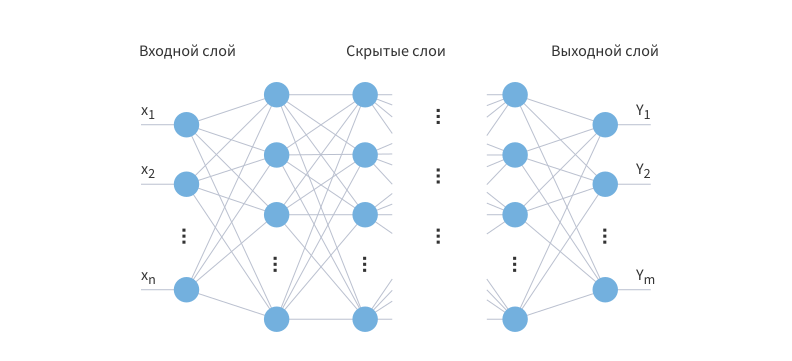
\includegraphics[scale=0.65]{multilayer-neural-net.png} 
  \caption{Схема многослойного перспетрона}
  \label{fig:analysis:multilayer-neural-net}
\end{figure}

В качестве активационных функций нейронов используются сигмоидальные: логистическая или гиперболический тангенс.

MLP показали возможность находить приближённые решения для чрезвычайно сложных задач. В частности, они являются
универсальным аппроксиматором функций, поэтому с успехом используются в построении регрессионных моделей.
Поскольку классификацию можно рассматривать как частный случай регрессии, когда выходная переменная категориальная,
на основе MLP можно строить классификаторы.

Пик популярности MLP в машинном обучении пришёлся на 1980-е годы в таких областях, как распознавание речи и
изображений, системах машинного перевода. Однако позднее они столкнулись с конкуренцией с другими технологиями
машинного обучения, такими, как машины опорных векторов. Интерес к многослойным персептронам вернулся благодаря
успехам глубокого обучения.

Радиально-симметричные функции – простейший класс функций. \linebreak В принципе, они могут быть использованы в разных моделях
(линейных и нелинейных) и в разных сетях (многослойных и однослойных). Традиционно термин RBF сети ассоциируется с
радиально-симметричными функциями в однослойных сетях, имеющих структуру, представленную на рисунке~\ref{fig:analysis:rbf-network}.

\begin{figure}[!ht]
  \centering
  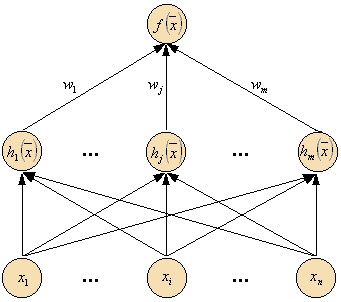
\includegraphics[scale=1]{rbf-network.png} 
  \caption{Схема RBF сети}
  \label{fig:analysis:rbf-network}
\end{figure}

То есть, каждый из n компонентов входного вектора подается на вход m базисных функций и их выходы линейно суммируются
с весами. \pagebreak

Таким образом, выход RBF сети является линейной комбинацией некоторого набора базисных функций:

\begin{equation}
  f(\overline{x}) = \sum_{j=1}^{m}{w_jh_j}
\end{equation}

Обобщенно-регрессионная нейронная сеть (GRNN) устроена аналогично вероятностной нейронной сети (PNN), но она
предназначена для решения задач регрессии, а не классификации. Обобщенная схема GRNN сети представлена на
рисунке~\ref{fig:analysis:grnn-network}. Как и в случае PNN-сети, в точку расположения каждого
обучающего наблюдения помещается гауссова ядерная функция. Мы считаем, что каждое наблюдение свидетельствует о
некоторой нашей уверенности в том, что поверхность отклика в данной точке имеет определенную высоту, и эта
уверенность убывает при отходе в сторону от точки. GRNN-сеть копирует внутрь себя все обучающие наблюдения и
использует их для оценки отклика в произвольной точке. Окончательная выходная оценка сети получается как взвешенное
среднее выходов по всем обучающим наблюдениям, где величины весов отражают расстояние от этих наблюдений до той точки,
в которой производится оценивание (и, таким образом, более близкие точки вносят больший вклад в оценку).

\begin{figure}[!ht]
  \centering
  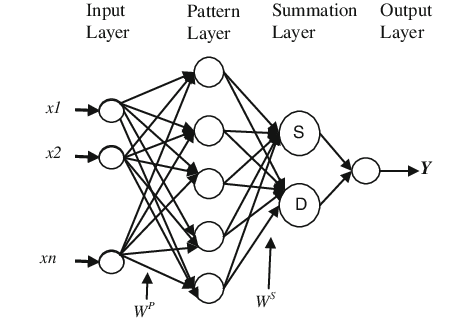
\includegraphics[scale=1.6]{grnn-network.png} 
  \caption{Схема GRNN сети}
  \label{fig:analysis:grnn-network}
\end{figure}

Первый промежуточный слой сети GRNN состоит из радиальных элементов. Второй промежуточный слой содержит элементы,
которые помогают оценить взвешенное среднее. Для этого используется специальная процедура. Каждый выход имеет в этом
слое свой элемент, формирующий для него взвешенную сумму. Чтобы получить из взвешенной суммы взвешенное среднее, эту
сумму нужно поделить на сумму весовых коэффициентов. Последнюю сумму вычисляет специальный элемент второго слоя.
После этого в выходном слое производится собственно деление (с помощью специальных элементов "деления"). Таким
образом, число элементов во втором промежуточном слое на единицу больше, чем в выходном слое. Как правило, в задачах
регрессии требуется оценить одно выходное значение, и, соответственно, второй промежуточный слой содержит два элемента.

Можно модифицировать GRNN-сеть таким образом, чтобы радиальные элементы соответствовали не отдельным обучающим
случаям, а их кластерам. Это уменьшает размеры сети и увеличивает скорость обучения. Центры для таких элементов
можно выбирать с помощью любого предназначенного для этой цели алгоритма (выборки из выборки, K-средних или Кохонена).

GRNN-сеть обучается почти мгновенно, но может получиться большой и медленной (хотя здесь, в отличие от PNN, не
обязательно иметь по одному радиальному элементу на каждый обучающий пример, их число все равно будет большим).
Как и сеть RBF, сеть GRNN не обладает способностью экстраполировать данные.

Проведенное сравнение полученных результатов(рис.~\ref{fig:analysis:comparing}),
полученных в статье~\cite{using_neural_engines} позволяет сделать выводы.

\begin{figure}[!ht]
  \centering
  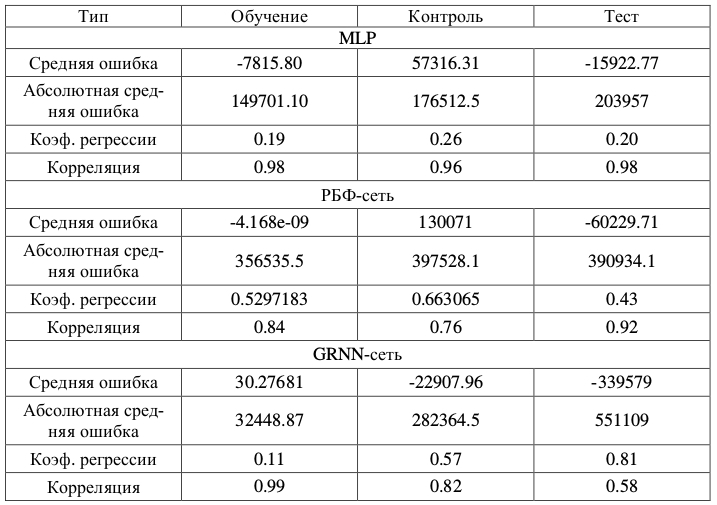
\includegraphics[scale=0.65]{comparing.jpg} 
  \caption{Сравнение полученных результатов}
  \label{fig:analysis:comparing}
\end{figure}

GRNN-сеть показала очень хорошие результаты на тестовой выборке, в то время как на тестовой выборке ее эффективность
оказалась значительно ниже, чем у прочих рассмотренных сетей. Наиболее вероятным здесь событием является нерешенная
проблема переобучения. То есть минимизировалась не та ошибка, которая ожидается от сети при подаче совершенно новых
значений. Другими словами, у данной сети отсутствует способность обобщать результаты работы на новые наблюдения.

РБФ-сеть не продемонстрировала высоких результатов, однако несомненным ее достоинством является более высокая скорость
обучения.

Многослойный персептрон является наиболее подходящим вариантом решения задачи определения стоимости жилых квартир.
Полученные данные позволяют с достаточной точностью прогнозировать стоимость квартир по заданным параметрам.

Достаточно высокая точность полученных результатов является следствием тщательно сформированной обучающей выборки.
Сравнение различных алгоритмов тренировки нейронной сети позволило выявить оптимальный алгоритм для имеющегося набора
данных. При этом, следует заметить, что все изучаемые алгоритмы продемонстрировали сравнительно высокую точность
предсказания результата.

Рассмотрены и реализованы 3 типа сетей: многослойный персептрон (MLP); сеть радиально-базисных функций (RBF);
обобщенно-регрессионная нейронная сеть (GRNN). Многослойный персептрон является наиболее подходящим вариантом решения
задачи определения стоимости жилых квартир. Полученные данные позволяют с достаточной точностью прогнозировать
стоимость квартир по заданным параметрам.
